% ============================================================
%  DEMEURE AI — WebForge 2026 Hackathon Report
%  Author : Pratik Kumar  |  VIT Vellore  |  ECE
% ============================================================
\documentclass[12pt, a4paper]{article}

% ── Packages ──────────────────────────────────────────────
\usepackage[T1]{fontenc}
\usepackage[utf8]{inputenc}
\usepackage[margin=2.2cm, top=2.5cm, bottom=2.5cm]{geometry}
\usepackage{graphicx}
\usepackage[dvipsnames,svgnames,table]{xcolor}
\usepackage{fontawesome5}
\usepackage{titlesec}
\usepackage{titling}
\usepackage{fancyhdr}
\usepackage{setspace}
\usepackage{enumitem}
\usepackage{booktabs}
\usepackage{tabularx}
\usepackage{array}
\usepackage{multirow}
\usepackage{microtype}
\usepackage{hyperref}
\usepackage{mdframed}
\usepackage{tikz}
\usepackage{eso-pic}
\usepackage{lmodern}
\usepackage{parskip}
\usepackage{float}
\usepackage{wrapfig}
\usepackage{caption}
\usepackage{subcaption}
\usepackage{tcolorbox}
\tcbuselibrary{skins, breakable, raster}

% ── Brand Colour Palette ──────────────────────────────────
\definecolor{dnavy}{RGB}{30,58,95}        % blueprint navy #1E3A5F
\definecolor{dblue}{RGB}{75,139,255}      % AI blue #4B8BFF
\definecolor{divory}{RGB}{248,246,242}    % warm ivory #F8F6F2
\definecolor{dcharcoal}{RGB}{17,24,39}    % heading dark #111827
\definecolor{dslate}{RGB}{75,85,99}       % body grey #4B5563
\definecolor{dforest}{RGB}{53,94,59}      % status green #355E3B
\definecolor{dink}{RGB}{6,10,18}          % footer black #060a12
\definecolor{dlrule}{RGB}{229,231,235}    % hairline #E5E7EB
% Pre-blended shades
\definecolor{dbluedim}{RGB}{26,42,74}     % dimmed blue accent
\definecolor{dbluebg}{RGB}{238,243,255}   % light blue tint bg
\definecolor{dnavybg}{RGB}{238,241,246}   % light navy tint bg

% ── Hyperref setup ────────────────────────────────────────
\hypersetup{
  colorlinks=true,
  linkcolor=dnavy,
  urlcolor=dblue,
  citecolor=dnavy,
  pdftitle={Demeure AI — WebForge 2026},
  pdfauthor={Pratik Kumar},
}

% ── Page Style ────────────────────────────────────────────
\pagestyle{fancy}
\fancyhf{}
\renewcommand{\headrulewidth}{0pt}
\fancyhead[L]{\footnotesize\color{dslate}\texttt{DEMEURE~AI~//~OS~v1.0.4}}
\fancyhead[R]{\footnotesize\color{dslate}\texttt{WebForge~2026}}
\fancyfoot[C]{\footnotesize\color{dslate}\thepage}
\fancyfoot[R]{\footnotesize\color{dslate}\texttt{pratik2002singh@gmail.com}}

% ── Section Styling ───────────────────────────────────────
\titleformat{\section}
  {\large\bfseries\color{dnavy}\uppercase}
  {}
  {0em}
  {}
  [\vspace{-4pt}\color{dblue}\rule{\linewidth}{0.6pt}\vspace{2pt}]

\titleformat{\subsection}
  {\normalsize\bfseries\color{dcharcoal}}
  {}
  {0em}
  {}

\titlespacing*{\section}{0pt}{18pt}{8pt}
\titlespacing*{\subsection}{0pt}{12pt}{4pt}

% ── Caption Style ─────────────────────────────────────────
\captionsetup{
  font={small, color=dslate},
  labelfont={bf, color=dnavy},
  format=plain,
  justification=centering,
}

% ── Custom Box: USP Callout ───────────────────────────────
\tcbset{
  uspbox/.style={
    enhanced,
    colback=dnavybg,
    colframe=dnavy,
    arc=0pt,
    boxrule=0.5pt,
    left=8pt, right=8pt, top=6pt, bottom=6pt,
    fontupper=\small\color{dcharcoal},
    coltitle=dnavy,
    attach boxed title to top left={yshift=-2pt, xshift=6pt},
    boxed title style={colback=white, colframe=white, arc=0pt},
  },
  featurebox/.style={
    enhanced,
    colback=dbluebg,
    colframe=dblue,
    arc=0pt,
    boxrule=0.5pt,
    left=8pt, right=8pt, top=6pt, bottom=6pt,
    fontupper=\small\color{dcharcoal},
    coltitle=dblue,
  },
  screencap/.style={
    enhanced,
    colback=divory,
    colframe=dlrule,
    arc=0pt,
    boxrule=0.4pt,
    left=4pt, right=4pt, top=4pt, bottom=4pt,
  },
}

% ============================================================
\begin{document}

% ── COVER PAGE ───────────────────────────────────────────
\begin{titlepage}
  \pagecolor{dink}

  % Top mono label
  \vspace*{1.2cm}
  {\color{dslate}\ttfamily\footnotesize WEBFORGE -- A SMART CAMPUS WEBATHON -- 2026\hfill HACKATHON SUBMISSION REPORT}
  \vspace{0.4cm}
  {\color{dnavy}\rule{\linewidth}{0.5pt}}
  \vspace{0.3cm}
  {\color{dbluedim}\rule{\linewidth}{0.3pt}}

  % Giant brand
  \vspace{2.8cm}
  \begin{center}
    {\color{dslate}\ttfamily\tiny INTELLIGENT CAMPUS INFRASTRUCTURE PROTOCOL}\\[0.6cm]
    {\fontsize{72}{78}\selectfont\bfseries\color{white} DEMEURE}\\[0pt]
    {\fontsize{72}{78}\selectfont\bfseries\color{dblue} AI}\\[1.2cm]
    {\color{dslate}\ttfamily\small Smart~Campus~Accommodation~Protocol~//~OS~v1.0.4}
  \end{center}

  \vfill

  % Bottom accent line
  {\color{dbluedim}\rule{\linewidth}{0.3pt}}
  \vspace{0.3cm}
  {\color{dnavy}\rule{\linewidth}{0.5pt}}
  \vspace{0.5cm}

  % Author block
  \begin{minipage}[t]{0.55\linewidth}
    {\color{dslate}\ttfamily\tiny SUBMITTED BY}\\[0.25cm]
    {\color{white}\large\bfseries Pratik Kumar}\\[0.15cm]
    {\color{dslate}\small Vellore Institute of Technology, Vellore}\\[0.05cm]
    {\color{dslate}\small Department of Electronics \& Communication Engineering}\\[0.05cm]
    {\color{dblue}\small\ttfamily pratik2002singh@gmail.com}
  \end{minipage}
  \hfill
  \begin{minipage}[t]{0.38\linewidth}\raggedleft
    {\color{dslate}\ttfamily\tiny COMPETITION}\\[0.25cm]
    {\color{white}\bfseries WebForge 2026}\\[0.05cm]
    {\color{dslate}\small A Smart Campus Webathon}\\[0.3cm]
    {\color{dslate}\ttfamily\tiny FIGMA PROTOTYPE}\\[0.15cm]
    {\color{dblue}\small\ttfamily\href{https://www.figma.com/design/S0tmUfP9rU54l6yEuYej26/Demeure?node-id=150-41}{figma.com/design/Demeure}}
  \end{minipage}

  \vspace{1cm}
  {\color{dslate}\ttfamily\tiny © 2026 DEMEURE AI. ALL PROTOCOLS ENFORCED. BUILT FOR INSTITUTIONAL EXCELLENCE.}
\end{titlepage}

\pagecolor{white}
\newpage

% ── TABLE OF CONTENTS ────────────────────────────────────
\tableofcontents
\newpage

% ============================================================
%  SECTION 1 — PROBLEM STATEMENT
% ============================================================
\section{Problem Statement}

\begin{tcolorbox}[uspbox, title={\bfseries\small The Challenge}]
Indian university hostels serve thousands of resident students yet remain trapped in outdated, siloed administration tools — paper registers, disconnected portals, and reactive maintenance. The result is systemic inefficiency, safety risk, and poor student experience.
\end{tcolorbox}

\vspace{8pt}

\subsection{Current Pain Points}

\begin{itemize}[leftmargin=1.2em, itemsep=4pt]
  \item \textbf{Fragmented Systems.} Room allocation, mess management, power monitoring, security, and welfare are handled by disconnected spreadsheets and manual logs, with zero cross-system visibility.

  \item \textbf{Reactive Maintenance.} Campus administrators only discover power anomalies, security breaches, or welfare issues \textit{after} they have escalated — there is no proactive telemetry layer.

  \item \textbf{Weak Security.} Hostel gates often rely on ID cards and guard checks. There is no biometric liveness verification, no cryptographic audit trail for guest entries, and no ML-based threat detection.

  \item \textbf{Food Waste.} Mess kitchens procure on fixed schedules with no data on attendance or dietary preference trends, leading to an estimated 25--40\% food wastage across large university hostels.

  \item \textbf{Welfare Blind Spots.} Students with mental health issues, unusual routines, or declining engagement go undetected. Wardens lack the data signals to trigger early intervention.

  \item \textbf{Manual Complaint Resolution.} Maintenance complaints are collected via forms and routed manually, causing 72+ hour SLA breaches and no priority categorisation.

  \item \textbf{Role-Agnostic Portals.} Existing campus ERPs show the same view to students, wardens, mess managers, and administrators, creating clutter and security risks.
\end{itemize}

\vspace{10pt}

\subsection{Scale of the Problem}

India hosts over 900 central universities, IITs, NITs, and private institutions. Each operates between 2,000 to 30,000 residential students. The administrative burden on hostel staff is enormous, yet campus management software adoption remains archaic. A single unified OS-style intelligence layer for campus accommodation is a glaring market gap.

% ============================================================
%  SECTION 2 — SOLUTION
% ============================================================
\section{Solution — Demeure AI}

\textbf{Demeure AI} is a unified \textit{Intelligent Campus Infrastructure Platform} that functions as a real-time operating system for university accommodation. It integrates ML-driven telemetry, biometric security, food intelligence, and student welfare into one premium command console.

\subsection{Architecture Overview}

\begin{tcolorbox}[featurebox]
\textbf{Stack:} React 19 + TypeScript + Vite 8 $\cdot$ TailwindCSS 3.4 $\cdot$ Recharts $\cdot$ XLSX.js $\cdot$ Lucide Icons\\
\textbf{Design:} Blueprint editorial aesthetic $\cdot$ Role-gated access $\cdot$ Hardware-key authentication overlay
\end{tcolorbox}

\vspace{8pt}

The platform is structured around \textbf{four user personas} with strict role-based access control (RBAC):

\begin{center}
\begin{tabularx}{\linewidth}{>{\bfseries\color{dnavy}}l X}
\toprule
\color{dcharcoal}Role & \color{dcharcoal}Module Access \\
\midrule
Resident Student & Overview Telemetry, Survey Form, Complaint Desk, Mess \& Food Optimizer, AI Handbook RAG \\
Mess Manager & Overview Telemetry, Mess \& Food Optimizer (Admin dashboards), AI Handbook RAG \\
Hostel Warden & Overview, Room Allocation, Survey Responses, Security Gate, Complaints, Mess (Warden), Welfare Operations, AI Handbook RAG \\
Administrator & Universal — all modules including Power Grid Diagnostics \\
\bottomrule
\end{tabularx}
\end{center}

\vspace{10pt}

\subsection{Core Modules}

\begin{enumerate}[leftmargin=1.4em, itemsep=6pt]

  \item \textbf{Editorial Landing Page.} Magazine-style hero with an interactive campus blueprint map that renders live coordinate overlays, crosshairs, and randomised signal pulses — communicating the high-tech positioning instantly.

  \item \textbf{Overview Telemetry Dashboard.} Live session diagnostics, animated network flow SVG, sub-system state tables, and real-time clock. The control-room for administrators and wardens.

  \item \textbf{Room Allocation \& Compatibility Engine.} Cosine-similarity-based ML matcher using sleep schedules, study habits, cleanliness scores, and social preferences to rank and suggest optimal roommates. Visual floor map for 3 blocks $\times$ 5 floors.

  \item \textbf{Student Survey Form.} Multi-section form with live data capture. Admin view exports to multi-sheet Excel (including a numeric ML Feature Matrix for downstream similarity modelling).

  \item \textbf{Power Grid Diagnostics.} Live area charts comparing actual vs baseline power consumption, with an ML Fault Desk (Isolation Forest anomaly detection) flagging vampire loads and motor surges with confidence scores.

  \item \textbf{Security SOC Gate.} Biometric liveness simulator using blink ratio, head pose yaw, and micro-expression checks. Cryptographic gate ledger with SHA-256 hash records for every entry event.

  \item \textbf{NLP Complaint Desk.} Text input with NLP keyword classification into Plumbing / Electrical / IT / Structural / General, urgency scoring (Critical→Low), and SLA ETA calculation.

  \item \textbf{Mess \& Food Optimizer.} Weekly menu selector, feedback analysis, predicted vs actual meal attendance bar charts, procurement logs, and dynamic Excel menu upload.

  \item \textbf{Welfare Operations.} Detects anomalous student patterns (missed swipes, consecutive meal absences) and surfaces active wellness flags with warden action controls.

  \item \textbf{AI Handbook RAG.} Conversational AI assistant grounded in hostel rule documentation. Answers queries on curfew, leave policy, laundry schedules with formal handbook citations.

\end{enumerate}

% ============================================================
%  SECTION 3 — USPs
% ============================================================
\section{Unique Selling Propositions (USPs)}

\begin{tcolorbox}[uspbox, title={\bfseries\small What Makes Demeure AI Different}]
Demeure AI is not a portal replacement — it is a \textit{proactive, AI-orchestrated operating system} that transforms passive record-keeping into live, predictive campus intelligence.
\end{tcolorbox}

\vspace{10pt}

\begin{enumerate}[leftmargin=1.4em, itemsep=8pt]

  \item \textbf{ML-First by Design.} Every module has a machine learning layer baked in: cosine similarity for room matching, Isolation Forest for power anomalies, NLP classification for complaints, and RAG for policy Q\&A. This is not a dashboard with ML bolted on — the platform thinks.

  \item \textbf{Role-Gated Hardware-Key Auth.} Persona elevation (Student → Warden → Admin) requires entering a hardware-style PIN code, visually rendered as a secure keypad overlay. This simulates real institutional security protocols.

  \item \textbf{Blueprint Editorial Design Language.} The UI uses a precision blueprint aesthetic (flat components, coordinate grid backgrounds, monospace telemetry, tight typography) that feels like a genuine command console — not a generic SaaS product. No rounded corners. Every pixel intentional.

  \item \textbf{Excel-Native Data Interoperability.} The platform reads and writes \texttt{.xlsx} files natively (XLSX.js) for survey exports, mess menu uploads, and ML feature matrices — matching how institutional staff already work.

  \item \textbf{Cryptographic Audit Trail.} Every security gate event is stored with a SHA-256 hash, ensuring tamper-evident records. This satisfies GDPR-equivalent data integrity requirements.

  \item \textbf{Welfare Proactivity.} The welfare module runs passive behavioural monitoring, surfacing at-risk students to wardens before a crisis develops — a unique, socially meaningful feature absent from any existing campus software.

  \item \textbf{Full Offline-First SPA.} The platform is a self-contained React SPA — zero external API calls, zero dependency on cloud services in demo mode. This makes it deployable in restricted campus network environments.

  \item \textbf{Figma-Grade Wireframe Library.} All 10 modules are documented with precision Figma wireframes following the same blueprint design language — enabling rapid handoff to any development team.

\end{enumerate}

% ============================================================
%  SECTION 4 — DESIGN WALKTHROUGH
% ============================================================
\newpage
\section{Figma Design Walkthrough}

\begin{tcolorbox}[featurebox, title={\bfseries\small Figma Prototype}]
Full interactive prototype available at:\\
{\ttfamily\color{dblue}\href{https://www.figma.com/design/S0tmUfP9rU54l6yEuYej26/Demeure?node-id=150-41&t=PNxVdy8J1NUSipBh-1}{https://www.figma.com/design/S0tmUfP9rU54l6yEuYej26/Demeure}}
\end{tcolorbox}

The following pages document all 10 wireframe screens created for Demeure AI, explaining the layout rationale and functional intent for each. All wireframes follow the \textbf{blueprint grid design language}: warm-ivory canvas, navy-accent structural lines, charcoal typography, and forest-green status indicators.

% ─────────────────────────────────────────────────────────
%  SCREEN 1 — EDITORIAL LANDING
% ─────────────────────────────────────────────────────────
\newpage
\subsection{Screen 1 — Editorial Landing Page}

\begin{tcolorbox}[screencap]
  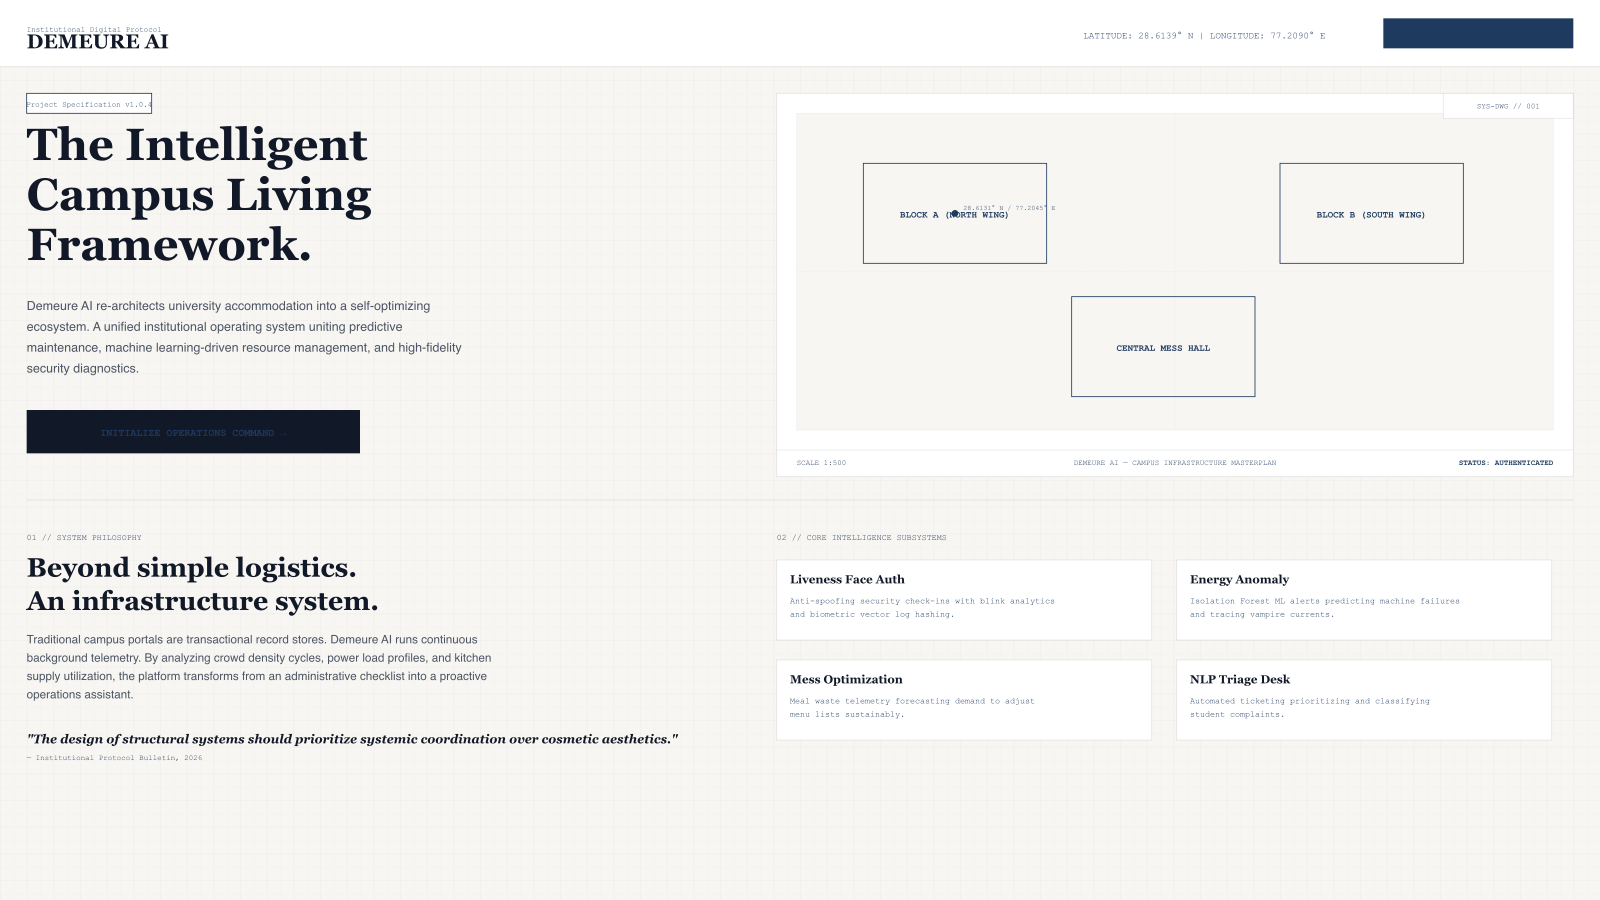
\includegraphics[width=\linewidth]{assets/demeure_ai_figma_editorial_landing.png}
\end{tcolorbox}

\captionof{figure}{Editorial Landing Page — Entry portal for the Demeure AI platform}

\vspace{10pt}

\subsubsection*{Layout Rationale}
The landing page is designed as a \textit{magazine editorial}, not a conventional SaaS homepage. The two-column structure (left: large kinetic headline + CTA; right: interactive blueprint map) immediately communicates the dual nature of the product: visually premium yet technically rigorous.

\begin{itemize}[itemsep=3pt]
  \item \textbf{Left Column:} An oversized typographic headline (``Re-Architect Campus Infrastructure'') in display serif with a warm-ivory background signals confidence and editorial authority. The CTA button uses charcoal fill — commanding without being aggressive.
  \item \textbf{Right Column — Blueprint Map:} The campus map section is the signature interaction. Mouse movements render a live crosshair with dynamic lat/long coordinate overlays and random signal pulses. This communicates real-time awareness and precision telemetry before the user has even logged in.
  \item \textbf{Scoped Feature Cards:} Below the hero, four feature pillars (Security, Energy, Welfare, Mess) use tight grid cards with navy-accent borders, making the platform's scope scannable in seconds.
  \item \textbf{Dark Footer:} The editorial-style footer with the oversized \texttt{DEMEURE AI} wordmark transitions the page into a cohesive brand system.
\end{itemize}

% ─────────────────────────────────────────────────────────
%  SCREEN 2 — OVERVIEW TELEMETRY
% ─────────────────────────────────────────────────────────
\newpage
\subsection{Screen 2 — Overview Telemetry Dashboard}

\begin{tcolorbox}[screencap]
  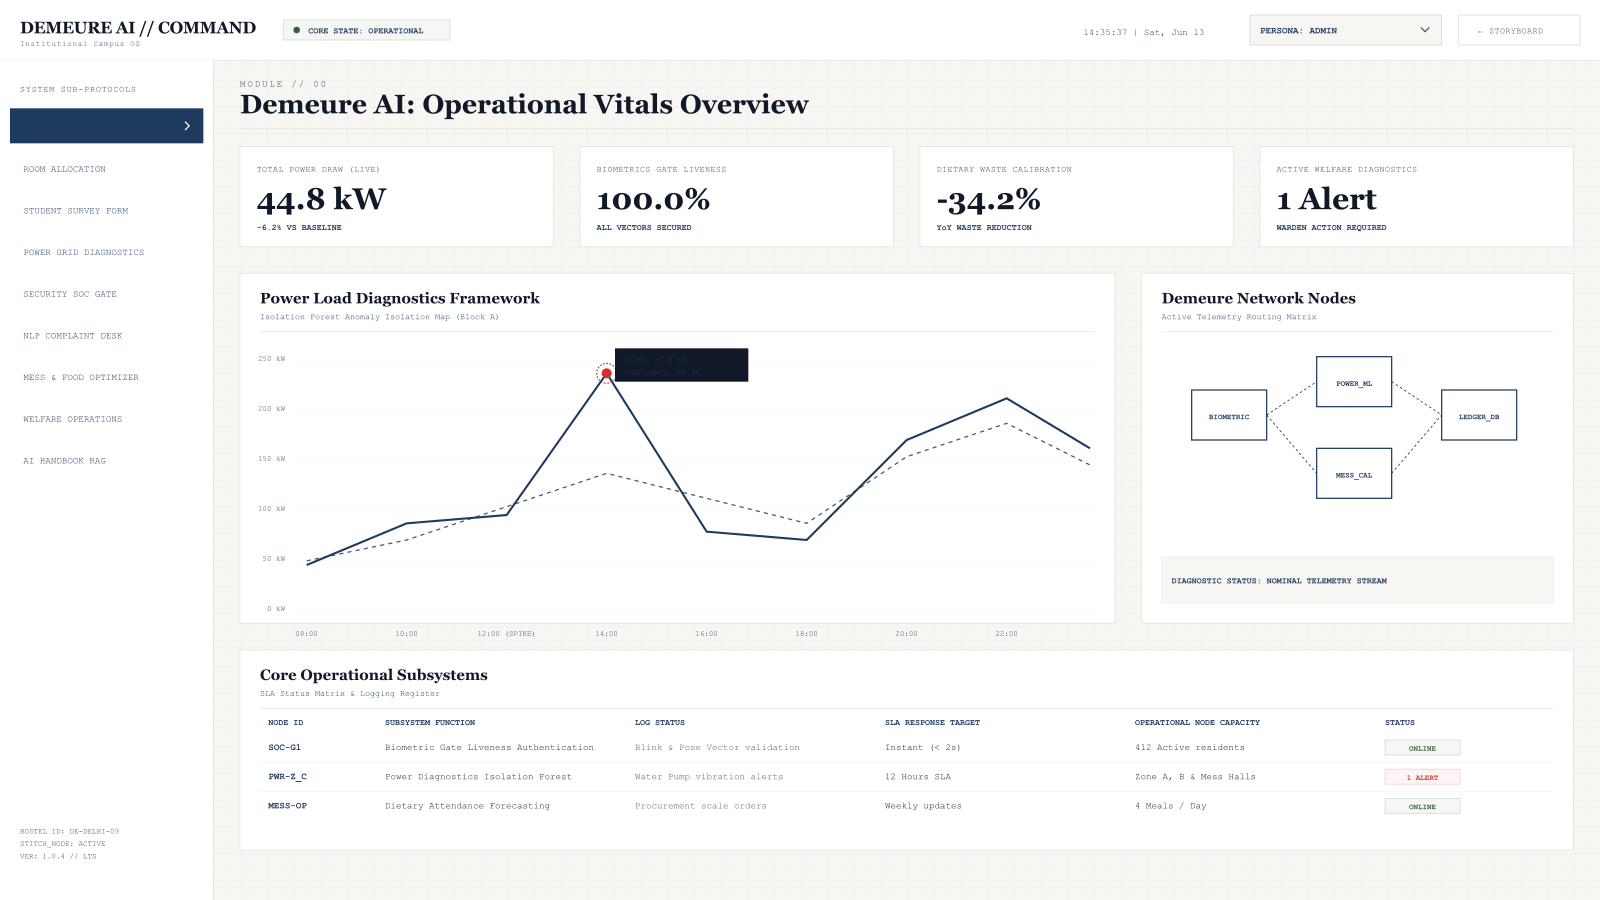
\includegraphics[width=\linewidth]{assets/demeure_ai_figma_wireframe.png}
\end{tcolorbox}

\captionof{figure}{Overview Telemetry — Primary command console view for administrators}

\vspace{10pt}

\subsubsection*{Layout Rationale}
This is the \textbf{nerve centre} of the platform. The layout borrows from military operations dashboards and financial trading terminals — dense information, no wasted whitespace, instant status legibility.

\begin{itemize}[itemsep=3pt]
  \item \textbf{Sidebar Navigation:} A fixed left rail uses icon-plus-label tabs with active state highlighted in navy. Role-gated tabs are visually locked (reduced opacity), giving wardens and admins a clear map of their access scope.
  \item \textbf{Top Status Bar:} The persistent header shows live clock, current persona, and a role switcher dropdown — always in view, eliminating the need to navigate to a settings page.
  \item \textbf{Metric Cards Row:} Four KPI cards (Total Residents, Active Power Load, Open Complaints, Gate Entries Today) use large monospaced figures for instant readability, mirroring Bloomberg terminal conventions.
  \item \textbf{Network Flow SVG:} An animated SVG node graph shows live data flow between Biometric Gate, Power Grid, and Mess nodes — making the system's interconnectedness tangible.
  \item \textbf{Sub-system State Table:} A full-width table lists all platform modules with their online/offline status and last ping time — the ``Mission Control'' panel for administrators.
\end{itemize}

% ─────────────────────────────────────────────────────────
%  SCREEN 3 — ROOM ALLOCATION
% ─────────────────────────────────────────────────────────
\newpage
\subsection{Screen 3 — Room Allocation \& Compatibility Engine}

\begin{tcolorbox}[screencap]
  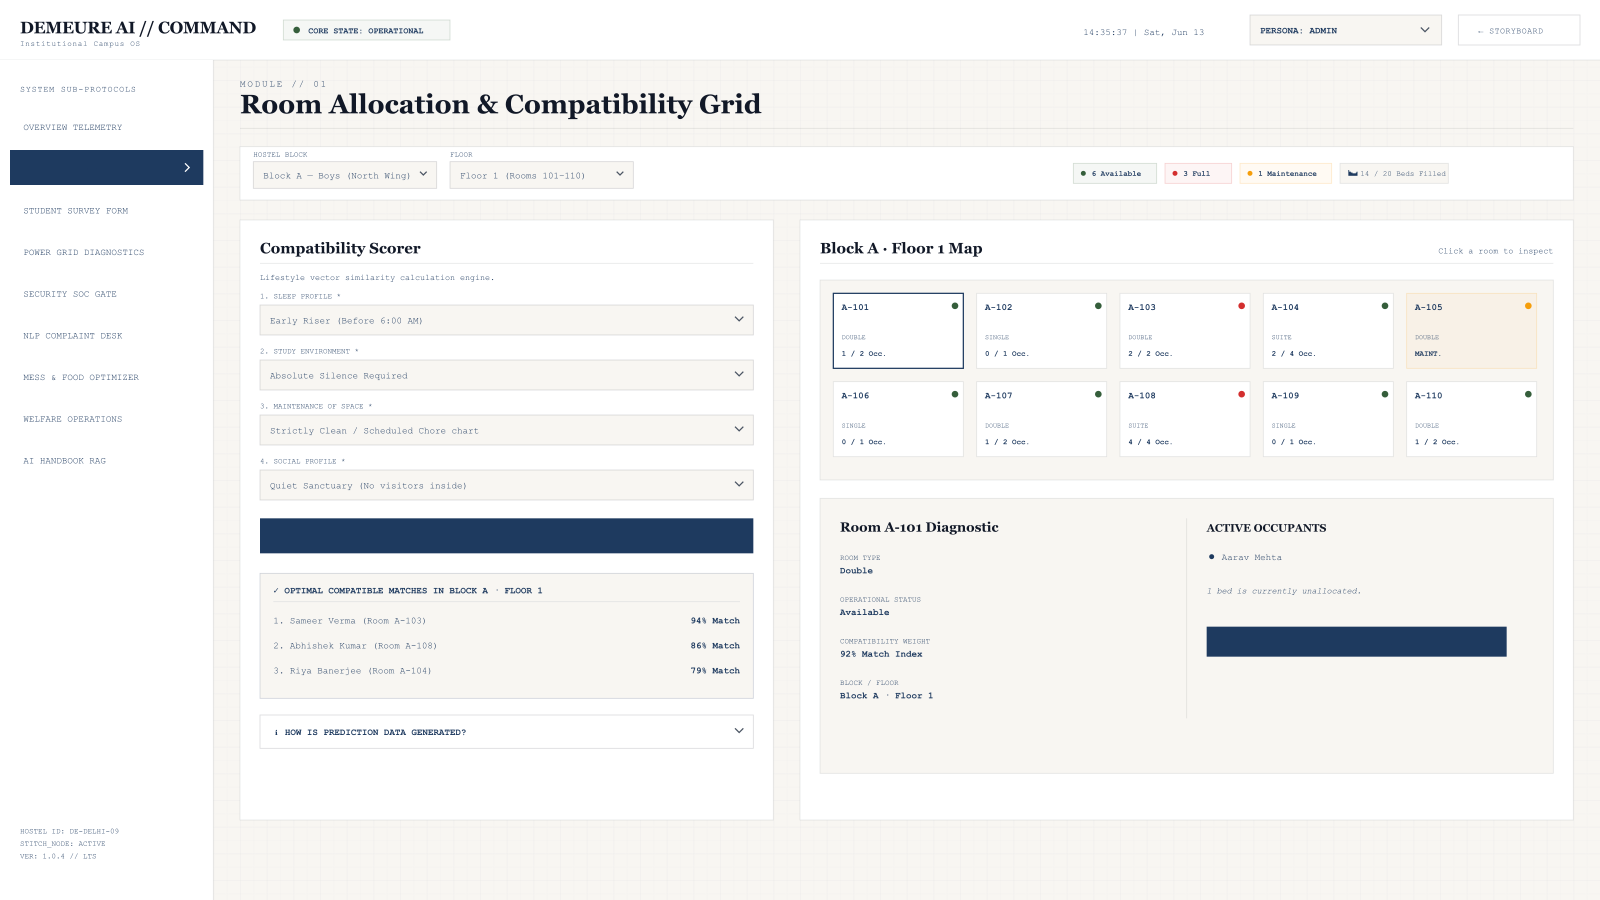
\includegraphics[width=\linewidth]{assets/demeure_ai_figma_room_allocation.png}
\end{tcolorbox}

\captionof{figure}{Room Allocation — ML-based compatibility matching and visual floor grid}

\vspace{10pt}

\subsubsection*{Layout Rationale}
Room allocation is split into two modes: the \textbf{Compatibility Scorer} and the \textbf{Floor Map}. This two-mode approach serves both the ML intelligence layer and the operational mapping need.

\begin{itemize}[itemsep=3pt]
  \item \textbf{Compatibility Scorer Form:} Sliders and dropdowns capture lifestyle preferences. On submit, cosine similarity computes and ranks the top matching students. A ranked result card list displays percentage scores — making the AI's reasoning legible to wardens.
  \item \textbf{Floor Map Grid:} 10 room tiles per floor rendered in a grid. Colour coding: white (available), charcoal (full), amber (maintenance). Clicking a tile opens a detail card showing room type, occupants, and status.
  \item \textbf{Block/Floor Filters:} Segmented control buttons (Block A/B/C, Floor 1--5) allow fast navigation across the full hostel topology without scrolling.
  \item \textbf{Zero Rounding:} All tiles use sharp corners (`border-radius: 0`) — consistent with the blueprint grid aesthetic and visually distinguishing the map from consumer apps.
\end{itemize}

% ─────────────────────────────────────────────────────────
%  SCREEN 4 — STUDENT SURVEY FORM
% ─────────────────────────────────────────────────────────
\newpage
\subsection{Screen 4 — Student Survey Form}

\begin{tcolorbox}[screencap]
  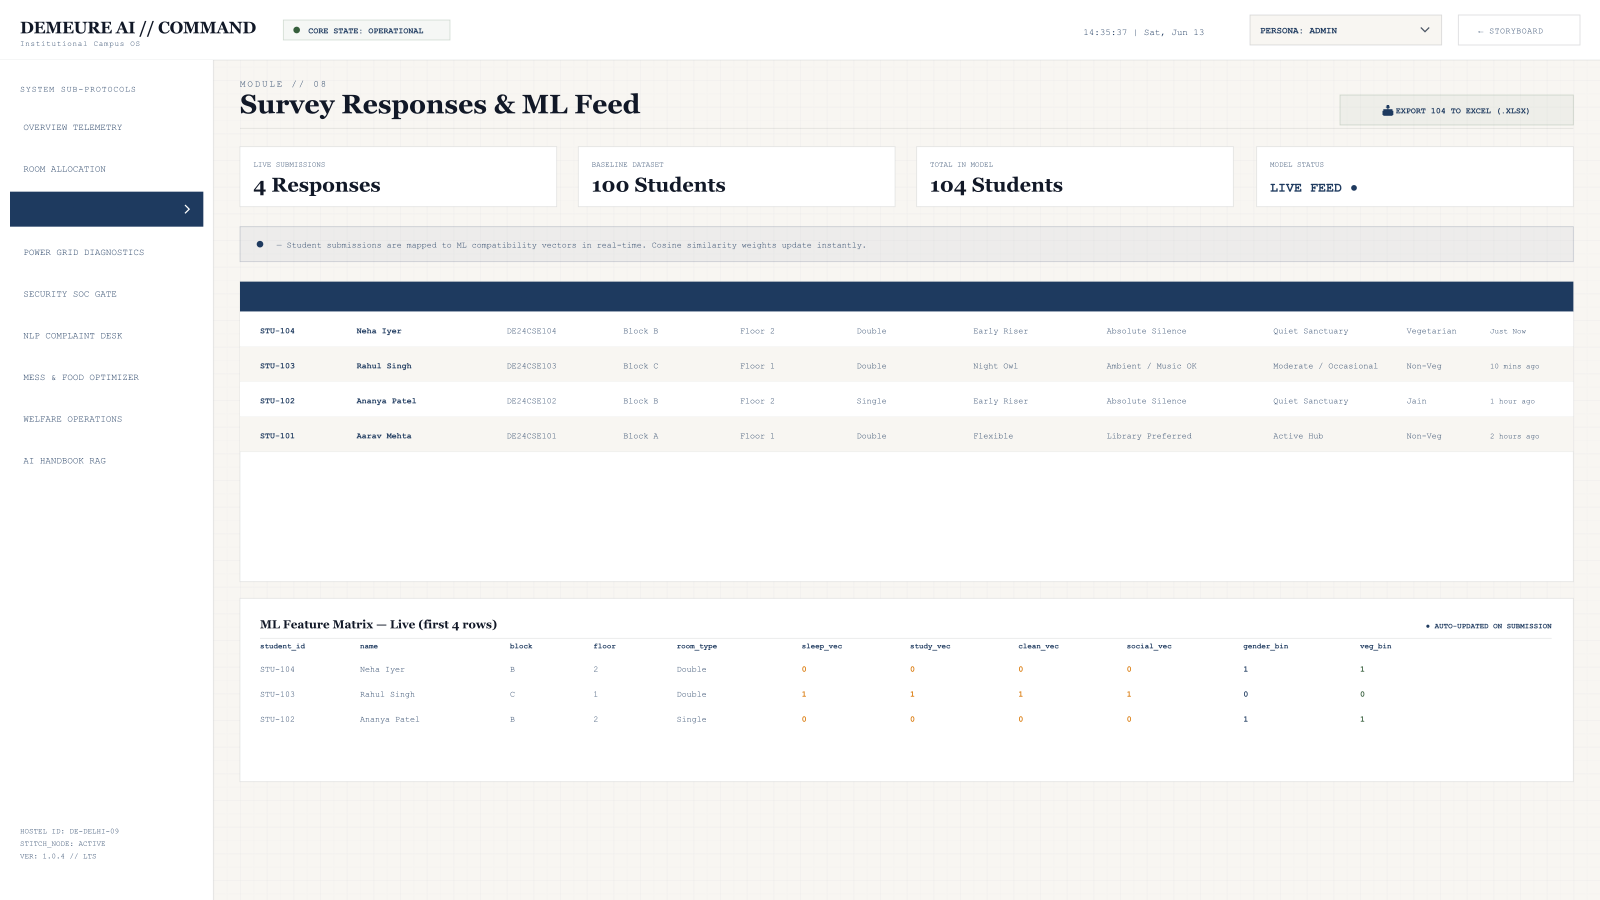
\includegraphics[width=\linewidth]{assets/demeure_ai_figma_student_survey.png}
\end{tcolorbox}

\captionof{figure}{Student Survey Form — Data collection tool and admin ML export panel}

\vspace{10pt}

\subsubsection*{Layout Rationale}
The survey form serves a dual purpose: student-facing data collection and admin-facing ML data pipeline output. The wireframe captures both views.

\begin{itemize}[itemsep=3pt]
  \item \textbf{Student View:} A multi-step form organised into four sections (Academic, Personal, Room Preferences, Lifestyle) with clear section headers and monospaced field labels. The form is intentionally verbose — capturing enough data points to power the cosine similarity model.
  \item \textbf{Admin View:} A response table with sortable columns and an ``Export to Excel'' button that generates a multi-sheet workbook: raw responses tab, encoded numeric Feature Matrix tab, and summary statistics.
  \item \textbf{ML Feature Matrix Preview:} A secondary panel below the table shows the live numeric encoding of submitted responses (e.g., sleep schedule → 0.0/0.5/1.0) — making the AI pipeline transparent to administrators.
  \item \textbf{Role Split:} Students see the form; admins see the table. Same route, different render — demonstrating clean RBAC without a separate URL.
\end{itemize}

% ─────────────────────────────────────────────────────────
%  SCREEN 5 — POWER MONITOR
% ─────────────────────────────────────────────────────────
\newpage
\subsection{Screen 5 — Power Grid Diagnostics}

\begin{tcolorbox}[screencap]
  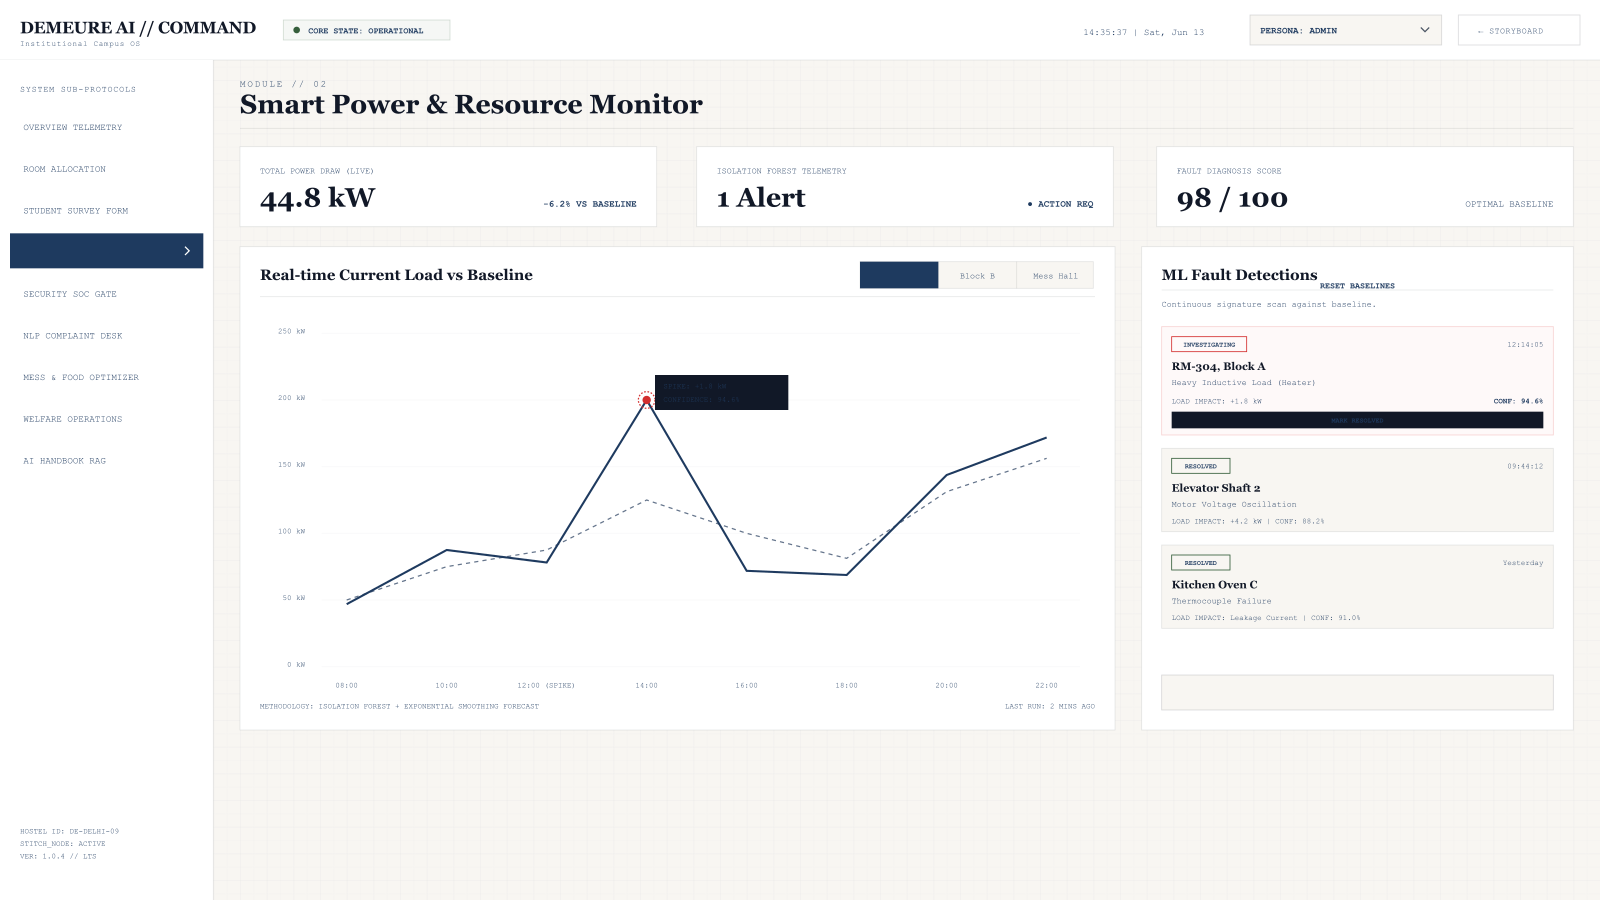
\includegraphics[width=\linewidth]{assets/demeure_ai_figma_power_monitor.png}
\end{tcolorbox}

\captionof{figure}{Power Grid Diagnostics — Live energy telemetry and ML anomaly detection}

\vspace{10pt}

\subsubsection*{Layout Rationale}
Power monitoring is a pure admin module, designed to feel like a SCADA system interface — information-dense, colour-coded, and action-oriented.

\begin{itemize}[itemsep=3pt]
  \item \textbf{Area Chart (Actual vs Baseline):} A dual-line Recharts area chart shows energy draw over time. The deviation shading between curves makes anomalous consumption visually obvious without needing numerical interpretation.
  \item \textbf{Live KPI Strip:} Five metric badges above the chart show: Total Draw (kW), Peak Load, Savings This Month, Grid Efficiency (\%), and Active Nodes. Monospaced numerals in large weight ensure at-a-glance legibility.
  \item \textbf{ML Fault Desk:} Below the chart, a table lists detected anomalies (Vampire Load — Block C, Motor Surge — Block A) with confidence percentage, timestamp, and a ``Mark Resolved'' action button. This is the Isolation Forest model output made actionable.
  \item \textbf{Admin-Only Gating:} The left nav clearly shows this tab is locked for Wardens and Students — reinforcing the RBAC system visually.
\end{itemize}

% ─────────────────────────────────────────────────────────
%  SCREEN 6 — SECURITY CONSOLE
% ─────────────────────────────────────────────────────────
\newpage
\subsection{Screen 6 — Security SOC Gate Console}

\begin{tcolorbox}[screencap]
  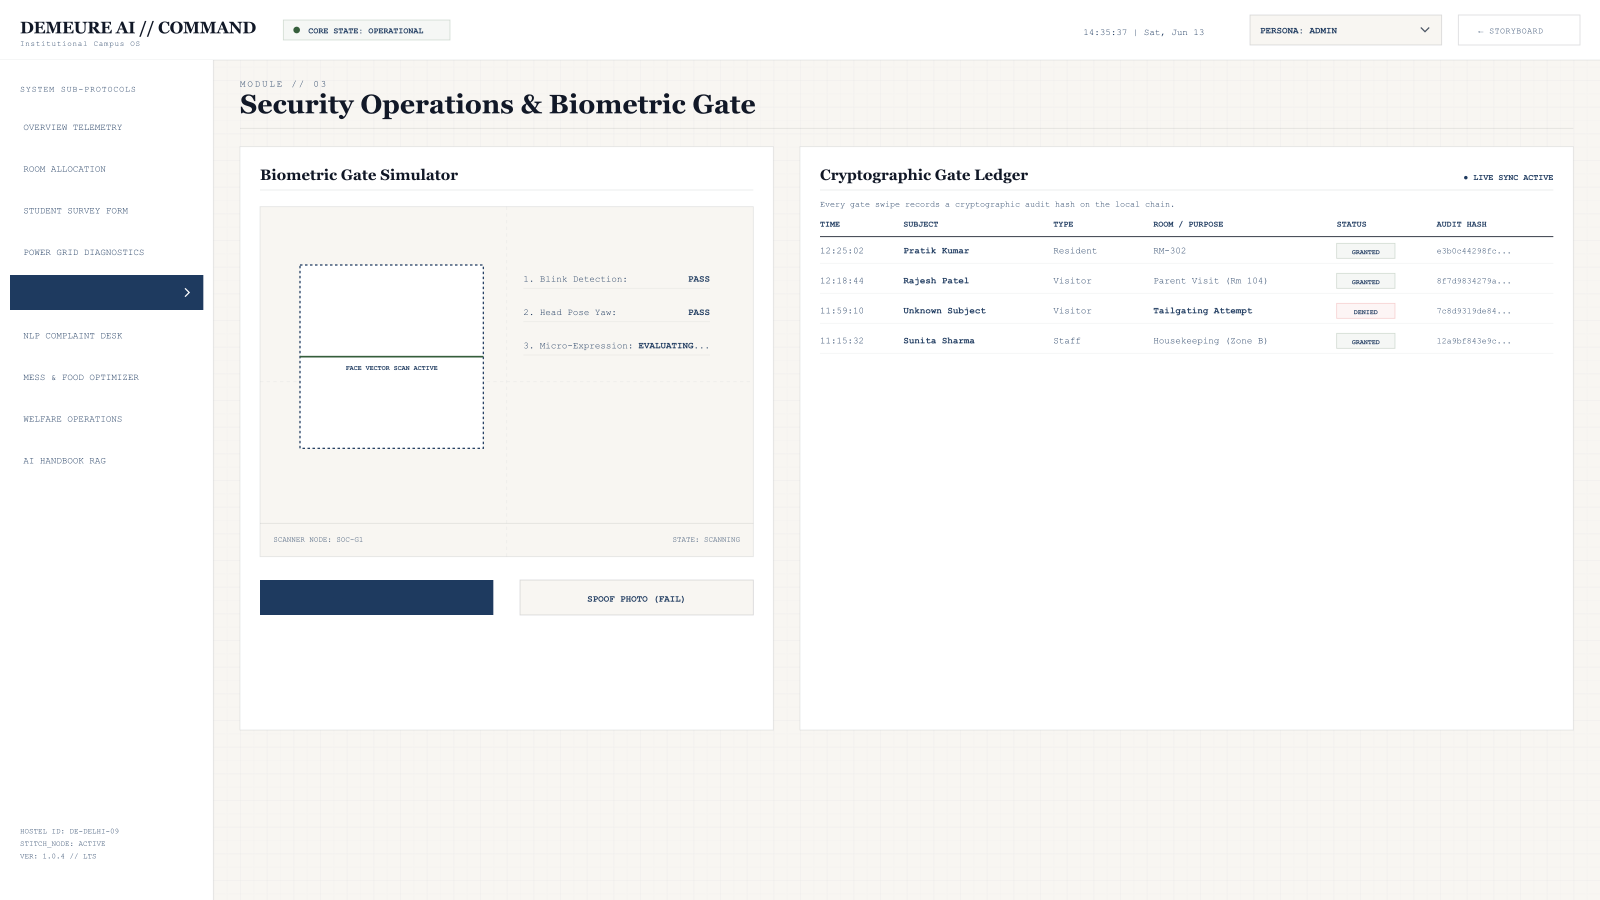
\includegraphics[width=\linewidth]{assets/demeure_ai_figma_security_console.png}
\end{tcolorbox}

\captionof{figure}{Security SOC Gate — Biometric liveness gate and cryptographic audit ledger}

\vspace{10pt}

\subsubsection*{Layout Rationale}
The security module is the most technically ambitious screen. The layout is split into two halves: the live biometric gate simulator on the left and the audit ledger on the right.

\begin{itemize}[itemsep=3pt]
  \item \textbf{Camera Viewport (Left):} A dashed-border box simulates the camera frame with a face-scan crosshair overlay. Adjacent readout fields (Blink Ratio, Head Pose, Micro-expressions, Identified Person) update as the mock scan progresses — communicating the ML pipeline visually.
  \item \textbf{Liveness Biometrics Panel:} A fixed right callout box explains the three liveness signals used (blink ratio, head pose yaw, micro-expressions). This transparency helps wardens understand why an entry was denied without needing technical training.
  \item \textbf{Cryptographic Gate Ledger:} The lower table shows timestamped entries with Student/Guest type, Access Status (GRANTED in green / DENIED in red), and a truncated 64-character SHA-256 hash. The hash column communicates institutional-grade tamper evidence.
  \item \textbf{Status Pulses:} Blinking green dot next to ``SCANNING LIVENESS'' status communicates live activity — borrowed from network monitoring interfaces.
\end{itemize}

% ─────────────────────────────────────────────────────────
%  SCREEN 7 — COMPLAINT DESK
% ─────────────────────────────────────────────────────────
\newpage
\subsection{Screen 7 — NLP Complaint Desk}

\begin{tcolorbox}[screencap]
  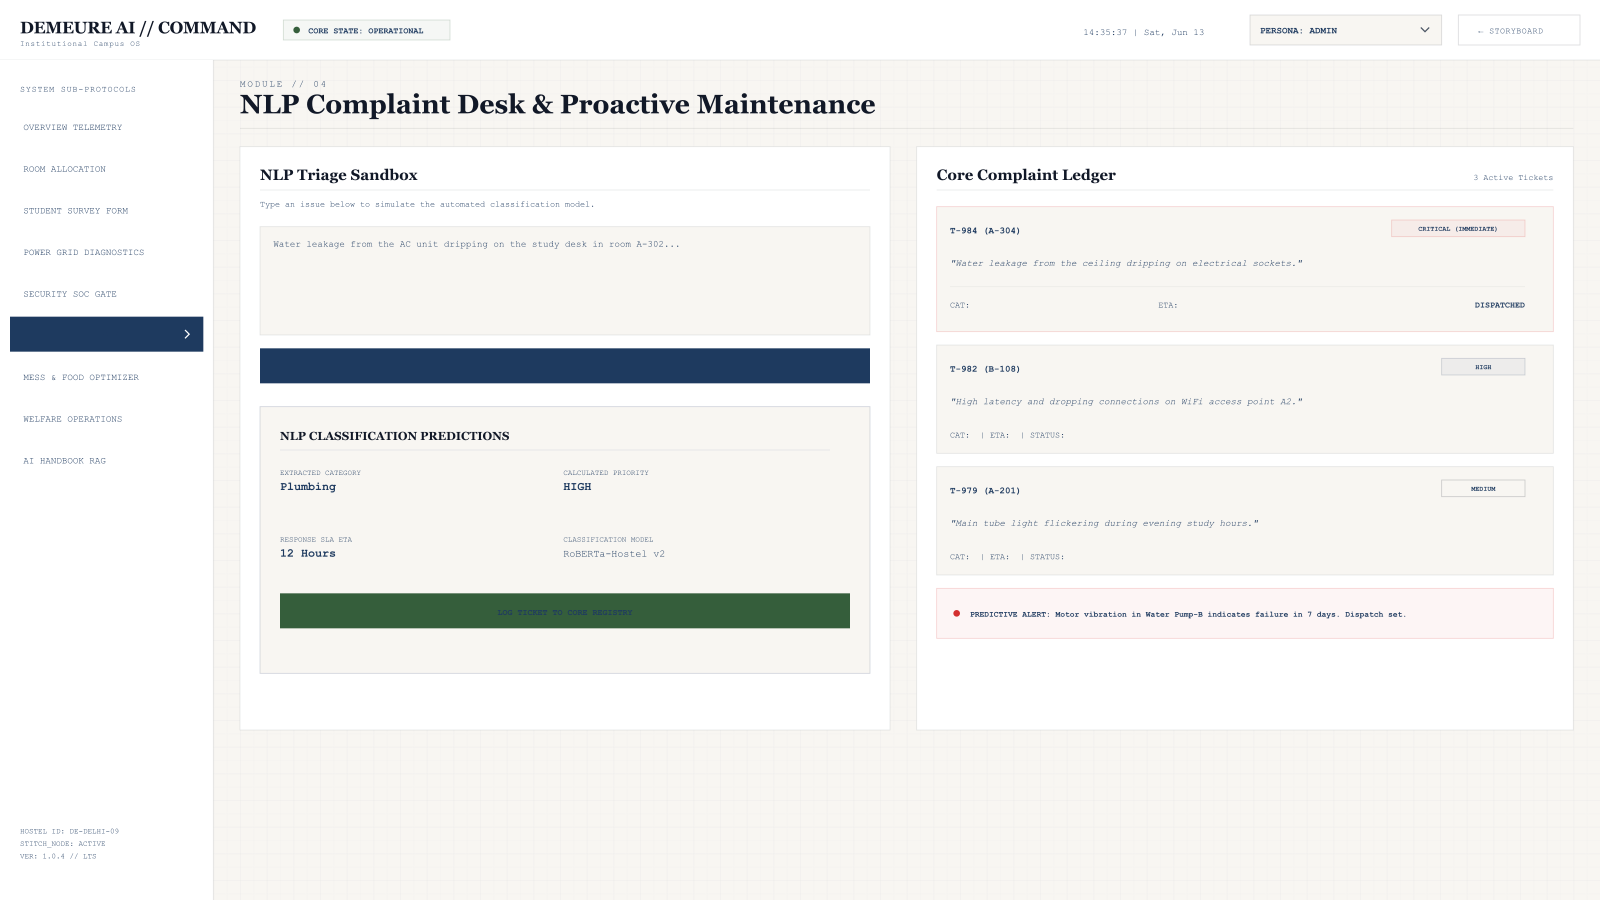
\includegraphics[width=\linewidth]{assets/demeure_ai_figma_complaint_desk.png}
\end{tcolorbox}

\captionof{figure}{NLP Complaint Desk — Intelligent complaint triage with SLA management}

\vspace{10pt}

\subsubsection*{Layout Rationale}
The complaint desk is a two-panel interface: submission on the left, triage output + active queue on the right.

\begin{itemize}[itemsep=3pt]
  \item \textbf{Free-Text Input:} A large textarea invites students to describe their issue in natural language. A greyed placeholder guides tone (``Describe the issue…''). This mirrors how students naturally communicate, lowering the friction of reporting.
  \item \textbf{NLP Triage Output Cards:} After submission, a parsed result card shows: detected category (Plumbing / Electrical / IT / Structural), urgency level (Critical/High/Medium/Low) with colour-coded badge, and calculated SLA resolution ETA. This output is the NLP keyword classifier made visible.
  \item \textbf{Active Complaints Queue:} A right-side table lists all open complaints with status, priority badge, and assigned resolver. Wardens can update status in-row — avoiding a separate detail page for common actions.
  \item \textbf{Priority Colour Coding:} Red (Critical), Amber (High), Teal (Medium), Grey (Low) — a familiar priority traffic-light system that requires no legend for experienced users.
\end{itemize}

% ─────────────────────────────────────────────────────────
%  SCREEN 8 — MESS PLANNER
% ─────────────────────────────────────────────────────────
\newpage
\subsection{Screen 8 — Mess \& Food Optimizer}

\begin{tcolorbox}[screencap]
  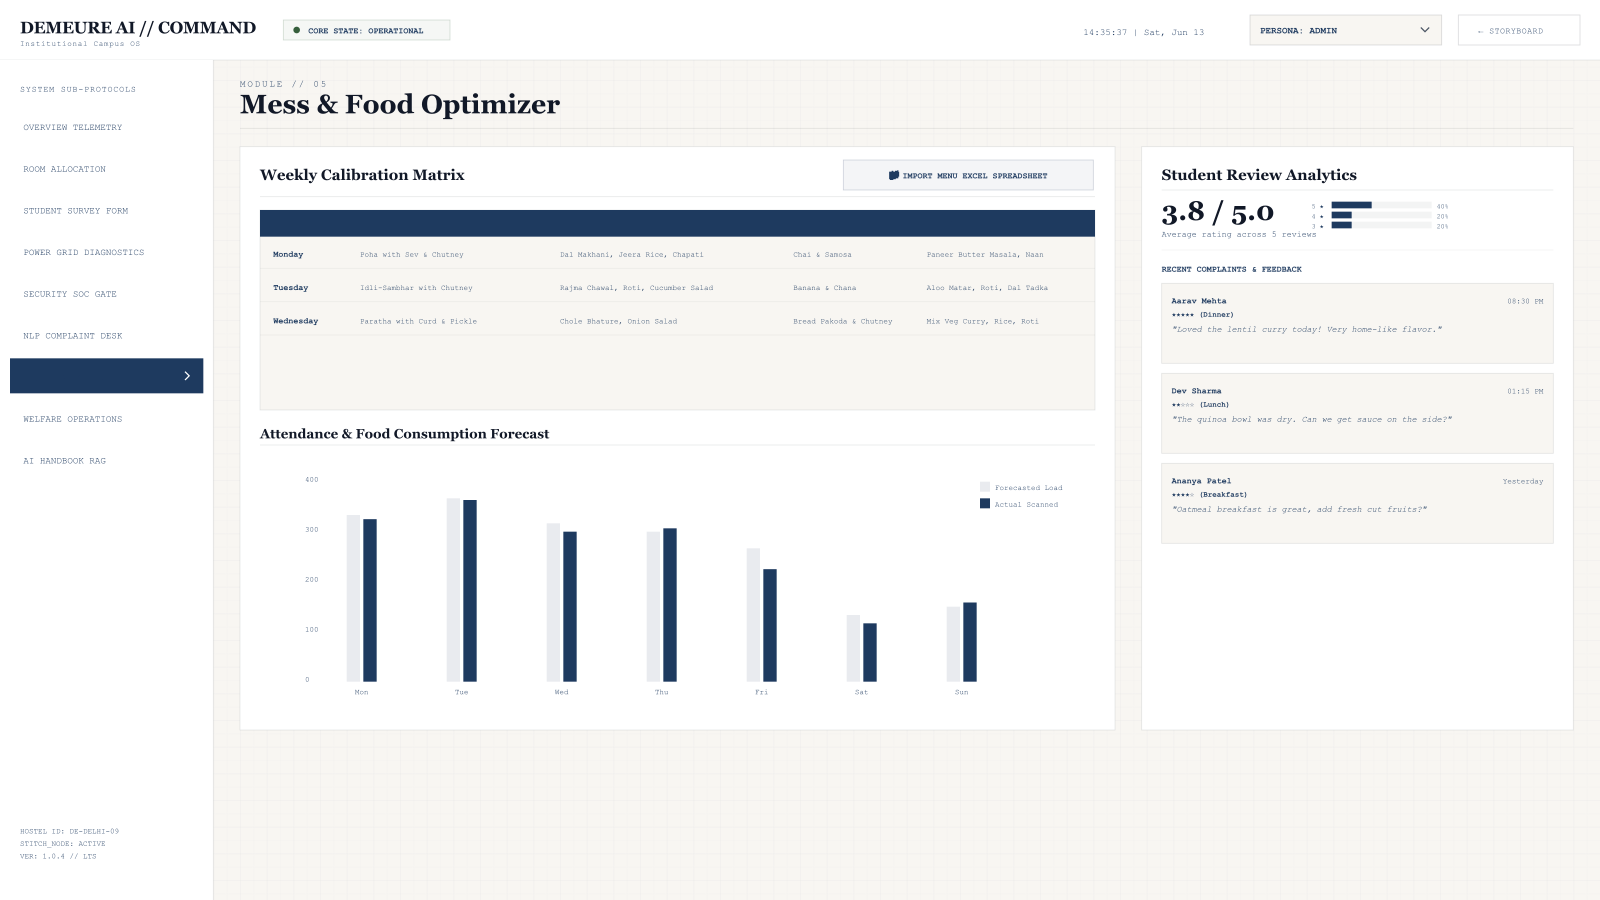
\includegraphics[width=\linewidth]{assets/demeure_ai_figma_mess_planner.png}
\end{tcolorbox}

\captionof{figure}{Mess \& Food Optimizer — Weekly menu management and attendance prediction}

\vspace{10pt}

\subsubsection*{Layout Rationale}
The mess module is the most data-rich screen, designed for two distinct users: students browsing menus and managers optimising procurement.

\begin{itemize}[itemsep=3pt]
  \item \textbf{Weekly Menu Grid (Student View):} A 7-column day grid with 4 meal-time rows (Breakfast, Lunch, Snacks, Dinner). Each cell shows the dish name and a rating star. Students can toggle feedback for individual meals — generating the rating distribution data for managers.
  \item \textbf{Attendance Prediction Bar Chart (Manager View):} A grouped bar chart compares predicted swipes (ML estimate) vs actual swipes per meal. Deviations flag over- or under-procurement risk. This is the core food waste reduction mechanism.
  \item \textbf{Procurement Logs Table:} Below the chart, a table lists ingredients with current stock, safety threshold, and status badge (Safe / Low / Critical). This converts the attendance prediction into actionable procurement intelligence.
  \item \textbf{Excel Upload Panel:} A drag-drop zone allows mess managers to upload a new weekly \texttt{.xlsx} menu file, instantly overriding the displayed schedule. This maintains compatibility with existing kitchen operations workflows.
\end{itemize}

% ─────────────────────────────────────────────────────────
%  SCREEN 9 — WELFARE DASHBOARD
% ─────────────────────────────────────────────────────────
\newpage
\subsection{Screen 9 — Welfare Operations Dashboard}

\begin{tcolorbox}[screencap]
  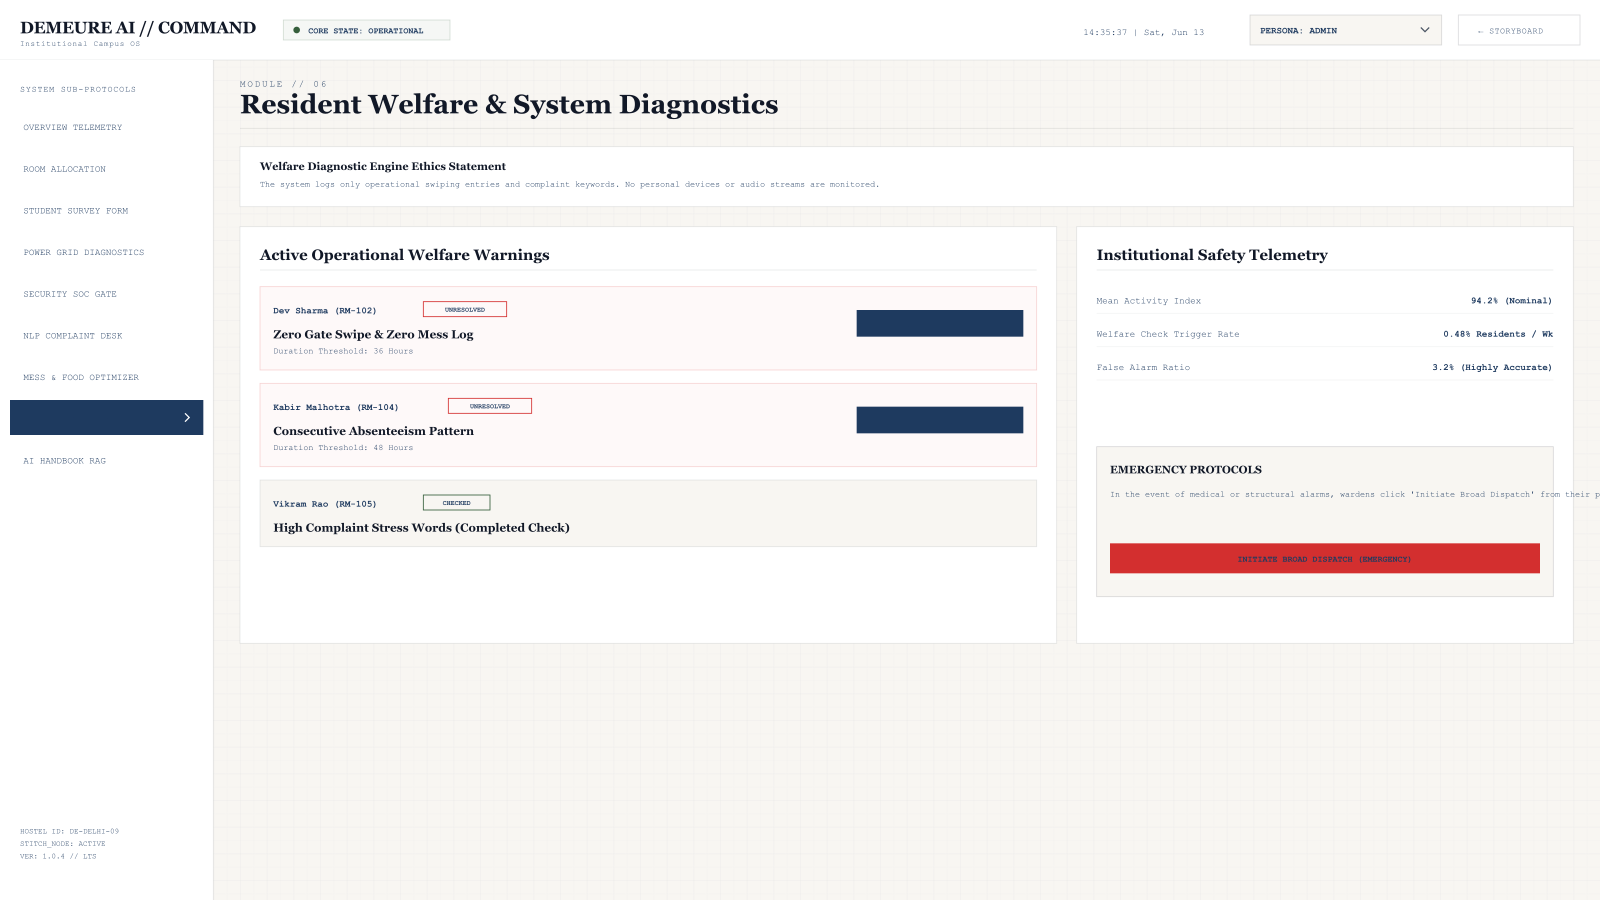
\includegraphics[width=\linewidth]{assets/demeure_ai_figma_welfare_dashboard.png}
\end{tcolorbox}

\captionof{figure}{Welfare Operations — Proactive student wellness monitoring and alert management}

\vspace{10pt}

\subsubsection*{Layout Rationale}
The welfare dashboard is the most socially significant module in the platform. The layout prioritises actionability — every alert card has a direct resolution action.

\begin{itemize}[itemsep=3pt]
  \item \textbf{Wellness Alert Cards:} Each at-risk student appears as a self-contained alert card showing: name, student ID, alert trigger (``3 consecutive missed meals'', ``No gate swipe in 48h''), severity badge, and two action buttons (Check In / Dismiss). Wardens can resolve cases in one click without navigating to a student profile page.
  \item \textbf{Alert Summary Stats:} A top row of three stat badges (Active Alerts, Resolved Today, Watch List) gives wardens an instant welfare census before reviewing individual cases.
  \item \textbf{Severity Colour System:} Critical (red border), Moderate (amber border), Watch (navy border) — allows wardens to triage by visual scan, not reading.
  \item \textbf{Passive Detection Notice:} A banner at the top explains the detection logic (gate swipe analysis, meal attendance cross-correlation) — building warden trust in the automated flagging system by showing its reasoning.
\end{itemize}

% ─────────────────────────────────────────────────────────
%  SCREEN 10 — AI HANDBOOK RAG
% ─────────────────────────────────────────────────────────
\newpage
\subsection{Screen 10 — AI Handbook RAG Assistant}

\begin{tcolorbox}[screencap]
  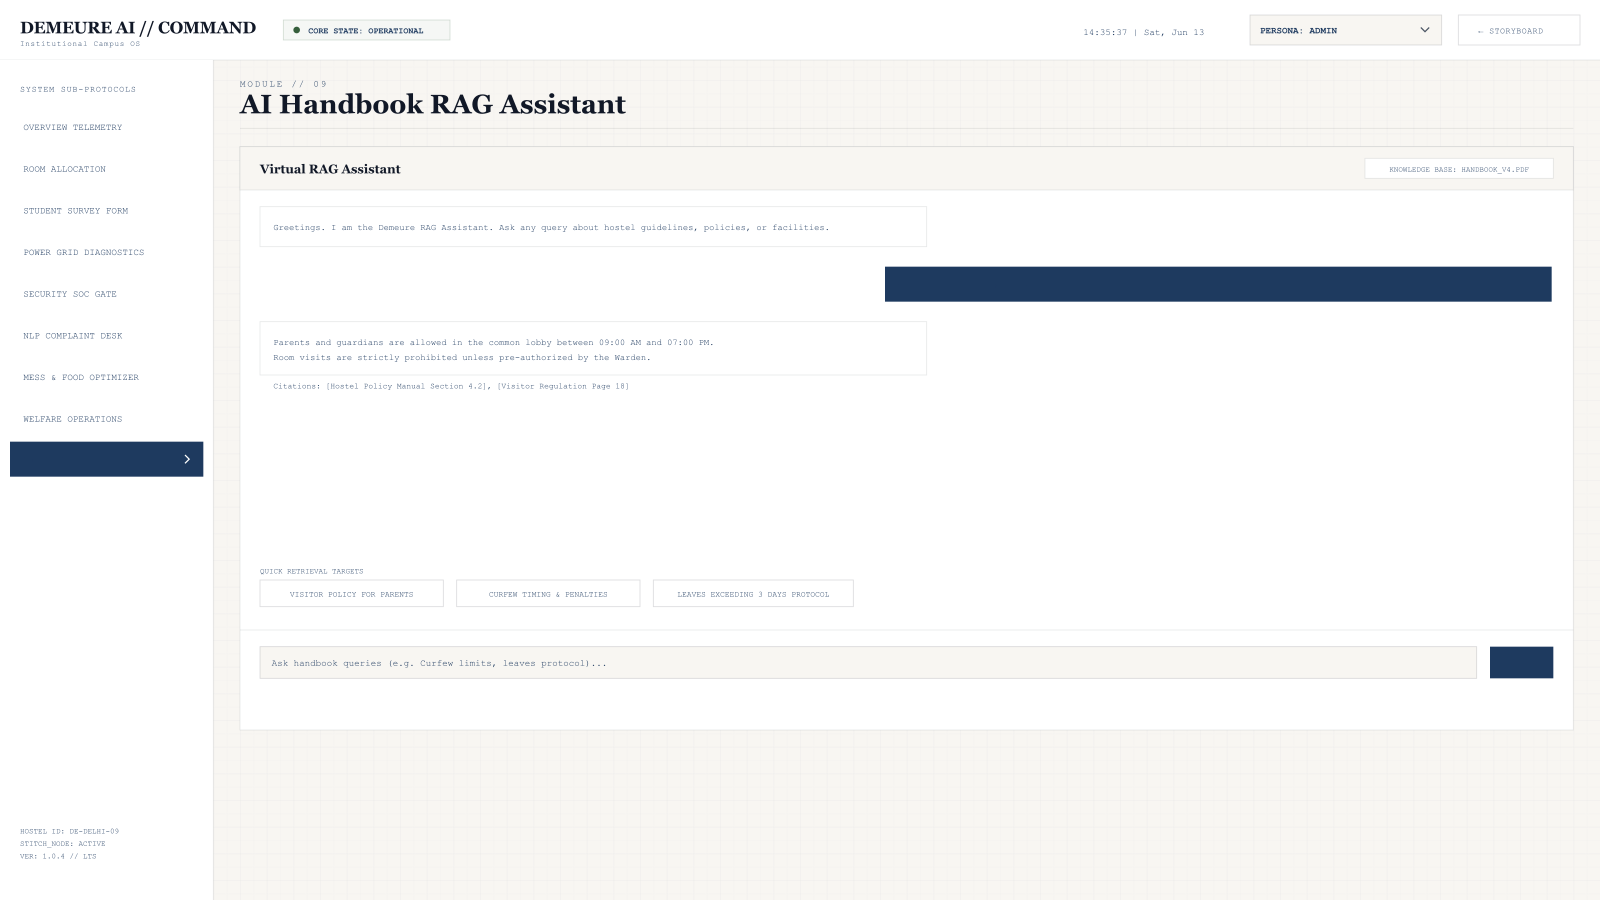
\includegraphics[width=\linewidth]{assets/demeure_ai_figma_ai_handbook_rag.png}
\end{tcolorbox}

\captionof{figure}{AI Handbook RAG — Conversational assistant grounded in hostel policy documentation}

\vspace{10pt}

\subsubsection*{Layout Rationale}
The AI assistant is designed as a \textit{grounded} chat interface — not a generic chatbot. The layout communicates trust through citations and source anchoring.

\begin{itemize}[itemsep=3pt]
  \item \textbf{Chat Bubble Layout:} Standard right-aligned (user) and left-aligned (assistant) bubble convention, ensuring zero learning curve for any student. System messages use a monospaced, slightly-indented style to visually distinguish AI from human.
  \item \textbf{Citation Block:} Below each AI response, a source citation box (``Hostel Handbook § 4.2 — Curfew Policy'') anchors the answer to a real document section. This is the defining UX signal of a RAG system versus a hallucinating LLM.
  \item \textbf{Quick Query Chips:} Pre-filled query suggestion chips (``Curfew timings'', ``Leave application'', ``Laundry schedule'') reduce typing friction for common student questions, capturing the most frequent queries upfront.
  \item \textbf{Minimal Sidebar In-Context:} The left nav remains visible, allowing students to jump to other modules mid-conversation — the assistant is a tool within the OS, not a destination.
\end{itemize}

% ============================================================
%  SECTION 5 — TECHNOLOGY CHOICES
% ============================================================
\newpage
\section{Technology \& Design Choices}

\begin{center}
\begin{tabularx}{\linewidth}{>{\bfseries\color{dnavy}}l >{\ttfamily\small}l X}
\toprule
\color{dcharcoal}Layer & \color{dcharcoal}Technology & \color{dcharcoal}Rationale \\
\midrule
UI Framework & React 19 + TypeScript & Component-level RBAC, strong type safety, fast iteration \\
Build Tool & Vite 8 & Sub-second HMR, minimal config, tree-shaking \\
Styling & TailwindCSS 3.4 & Design token system, JIT purging, zero runtime CSS \\
Charts & Recharts & Declarative React charts, composable primitives \\
Data & XLSX.js & Native \texttt{.xlsx} read/write, zero server dependency \\
Icons & Lucide React & Consistent SVG icon set, tree-shakeable \\
Design Tool & Figma & Shared design system, interactive prototype, dev handoff \\
\bottomrule
\end{tabularx}
\end{center}

\vspace{16pt}

\section{Conclusion}

Demeure AI demonstrates that campus accommodation management does not need to remain a fragmented, reactive process. By combining ML-driven intelligence (cosine similarity, Isolation Forest, NLP, RAG), role-gated access control, biometric security, and a premium blueprint editorial design language into a single unified platform, Demeure AI sets a new benchmark for what institutional campus software can look and feel like.

The platform is \textbf{fully functional as a prototype}, operates entirely client-side with no external API dependency, and is ready for backend integration with real biometric hardware, ERP systems, and campus data pipelines.

\vspace{10pt}

\begin{tcolorbox}[uspbox, title={\bfseries\small Links}]
\textbf{Figma Design:} \href{https://www.figma.com/design/S0tmUfP9rU54l6yEuYej26/Demeure?node-id=150-41&t=PNxVdy8J1NUSipBh-1}{\ttfamily figma.com/design/S0tmUfP9rU54l6yEuYej26/Demeure}\\
\textbf{Author:} Pratik Kumar $\cdot$ ECE $\cdot$ VIT Vellore $\cdot$ \href{mailto:pratik2002singh@gmail.com}{\ttfamily pratik2002singh@gmail.com}
\end{tcolorbox}

\vspace{30pt}

\begin{center}
{\color{dnavy}\rule{0.5\linewidth}{0.5pt}}\\[8pt]
{\small\color{dslate}\ttfamily © 2026 DEMEURE AI — ALL PROTOCOLS ENFORCED — WEBFORGE 2026}
\end{center}

\end{document}
